% Marius: I think this part should establish a little more on the motivation and introduction part. Right now I think the reader has no idea what this is about if they were never exposed to the project before.

We assumed that we might not have an access to the real time data and the only data that will be provided to us might be a batch data. For that reason and to be able to work in parallel the system architecture in our project is composed of 2 approaches: \textbf{fixed} and \textbf{stream}. \\
In the fixed approach we will train and test multiple machine learning models, not to wait for whole real time infrastructure.
In stream approach we will create the whole streaming infrastructure and than reuse already prepared, trained and tested models from the fixed approach.\\
At the end we received the following system architecture fig. \ref{fig:architecture}. In the final architecture we are using previously gathered data(fixed) to train the ML models. Those trained models will be used for a real time streamed data in which we will try to detect anomalies.  

\subsection{Brief, high level description of the system architecture - Jacek}
\begin{itemize}
\item \textbf{In a fixed approach} we use fixed chunks of data provided by BMW to train the models deployed in AWS SageMaker. 
\item \textbf{In a stream approach} we assumed that the data might come from multiple sources. We gather these data using Kinesis Stream as a queue. Then using a Amazon Simple Notification Service (SNS) lambdas is triggered. This lambdas feed the models with incoming data. In case of anomaly detection feeding lambda is triggering different notification functions using SNS topic to inform user that anomaly has been detected.
\end{itemize}
% Marius: Whats a lambda? Whats SNS?

A more detailed description is provided in a following chapter.
\begin{figure}[h]
    \centering
    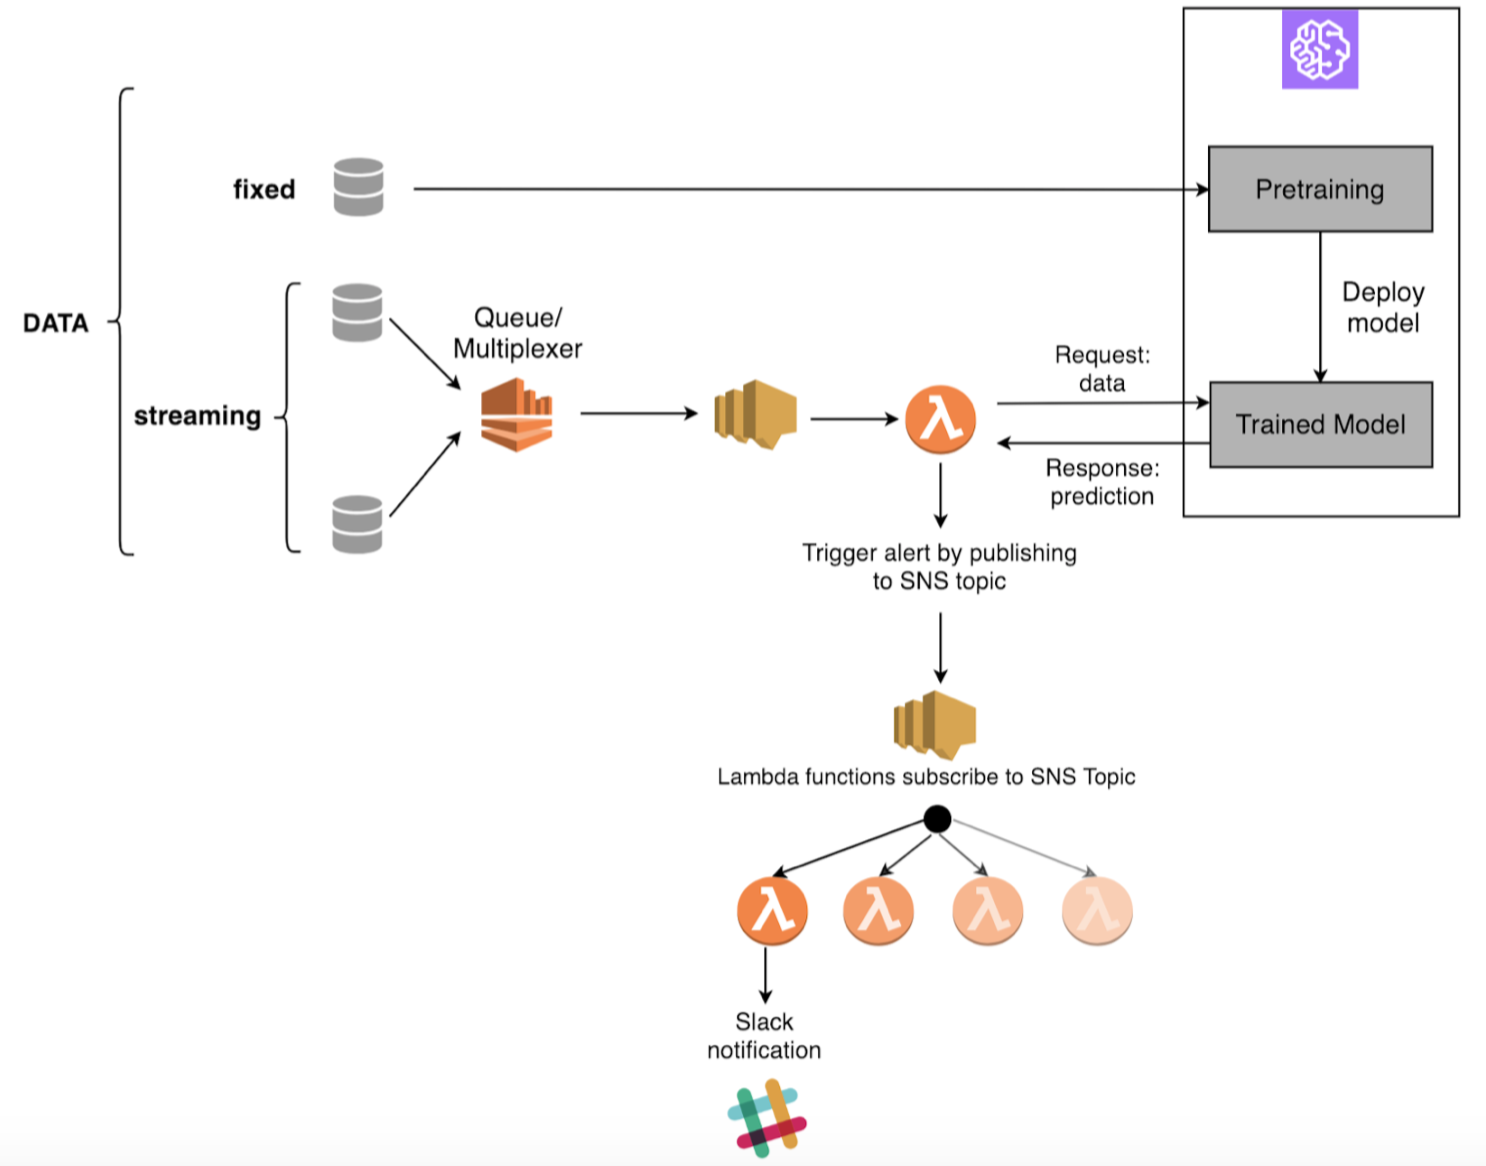
\includegraphics[width=0.8\textwidth]{images/sys-architecture.png}
    \caption{System architecture schema}
    \label{fig:architecture}
\end{figure}
    
